%       File: VTthesis_template.tex
%     Created: Thu Mar 24 11:00 AM 2025 EDT
%     Last Change: August 15, 2025
%     Author: Priyatam Annambhotla, VT
%	  With modifications by Carrie Cross, Robert Browder, and LianTze Lim. 
%
% This template is designed to operate with XeLaTeX.
%
% All elements in the Title, Abstract, and Keywords MUST be formatted as text and NOT as math.
%
%Further instructions for using this template are embedded in the document. Additionally, there are comments at the end of the file that give suggestions on writing your thesis.  
%
%In addition to the standard formatting options, the following options are defined for the VTthesis class: proposal, prelim, doublespace, draft. 

\documentclass[doublespace,nopageskip]{VTthesis} % nopageskip - Removes arbitrary blank pages.
%Remove "draft" from \documentclass to remove draft watermark and to display figures you've created.

% Using the following header instead will create a draft copy of your thesis
%\documentclass[doublespace,draft]{VTthesis}

% The lipsum package is just included to put dummy text in the document in order to demonstrate page headers and table of contents behavior. You should remove it once you begin writing your actual thesis or dissertation.
\usepackage{lipsum}
\usepackage{graphicx}
\usepackage{booktabs}
\usepackage{tabularx}
\usepackage{algorithm}
\usepackage{algorithmic}

% Title of your thesis
\title{PIN: Protocol Buffer-Based Input Normalization for Program Analysis and Testing}

% You should include 3-5 keywords, separated by commas
\keywords{Program Analysis, Input Normalization, Protocol Buffers, C Program Transformation, Fuzzing, Static Analysis}

% Your name, including middle initial(s)
\author{Priyatam Annambhotla}

% Change this to your program, e.g. Physics, Civil Engineering, etc.
\program{Electrical and Computer Engineering} 

% Change this to your degree, e.g. Master of Science, Master of Art, etc.
\degree{Master of Science} 

% This should be your defense date:
\submitdate{October 15, 2025} 

% Committee members. Only have five readers and one chair available.
% Only use the ones you need and don't include the ones you don't need.
% You can also declare a Co-advisor. Per the VT ETD standards, 
% you should not include titles such as Dr. or Professor, but can list educational 
% qualifications after the name (i.e., John Doe, MFA or Jane Smith, PhD)
% Names should appear as they do in ESS/Banner/HokieSpa, including middle initials.
\principaladvisor{Binoy Ravindran}
\coadvisor{Zhoulai Fu}
\firstreader{TBD}
\secondreader{TBD}
\thirdreader{TBD}
%\fourthreader{Fourth Committee Member}
%\fifthreader{Fifth Committee Member}

% The dedication and acknowledgement pages are optional. Comment them out to remove them.
\dedication{This is where you put your dedications.}
\acknowledge{This is where you put your acknowledgments.}

% The abstract is required.
\abstract{This thesis presents PIN (Program Input Normalization), a toolchain that transforms C programs so they accept standardized Protocol Buffer inputs. PIN automatically extracts input structures, synthesizes schemas, and emits nanopb-based wrappers that reconstruct the original calling convention. A new pointer management strategy classifies pointer parameters (scalars, slices, structs, chains) and generates helper messages and reconstruction logic for both the nanopb wrapper and a C++ reference runner. To reason about semantic equivalence when fuzzing arbitrary byte streams, we adopt an \emph{equivalence modulo input validation} (EMI) policy: only inputs that decode into values satisfying the original function's preconditions are compared across implementations. Evaluation on coreutils, Toyota ITC, and custom pointer-heavy benchmarks shows that PIN covers 8/9 pointer fixtures end-to-end, improves test generation coverage, and exposes remaining gaps (struct slices, opaque pointers). The approach bridges manual input crafting and automated analysis by providing a scalable, semantics-aware normalization pipeline.}
%\abstract{\lipsum [1-4]}

% The general audience abstract is required. There are currently no word limits.
\abstractgenaud{Software testing is crucial for ensuring programs work correctly, but creating the right test inputs for C programs is often difficult and time-consuming. This research introduces PIN, a tool that automatically converts C programs to accept standardized inputs using Google's Protocol Buffers. PIN not only learns the basic shapes of inputs, it also understands pointers---the links C programs use to reference data in memory---and regenerates them safely for testing. Because random byte streams can describe nonsense inputs, we compare behaviour only when the decoded data meets the program's expectations, an approach known as ``equivalence modulo input validation.'' In effect, PIN builds a universal adapter that lets testing tools communicate with complex C software while respecting the program's rules. The tool successfully handles real-world programs and pointer-heavy examples, making systematic testing more practical for software companies, security researchers, and anyone who needs reliable C code.}

\begin{document}
% The following lines set up the front matter of your thesis or dissertation and are required to ensure proper formatting per the VT ETD standards. 
  \frontmatter
  \maketitle
  \tableofcontents

% The list of figures and tables are now optional per the official ETD standards.  Unless you have a very good reason for removing them, you should leave these lists in the document. Comment them out to remove them.
	\listoffigures
	\listoftables
    \printnomenclature %Creates a list of abbreviations. Comment out to remove it. 

% Abbreviations used throughout the thesis
\nomenclature{PIN}{Program Input Normalization}
\nomenclature{EMI}{Equivalence Modulo Input Validation}
\nomenclature{AST}{Abstract Syntax Tree}
\nomenclature{PB}{Protocol Buffers serialization format}
\nomenclature{NPB}{Nanopb embedded Protocol Buffers runtime}
\nomenclature{CLI}{Command-Line Interface}

% The following sets up the document for the main part of the thesis or dissertation. Do not comment out or remove this line.
	\mainmatter

	%now go ahead and start writing your thesis
	\chapter{Introduction} \label{ch:introduction}
	
	Software testing and program verification remain among the most critical challenges in software engineering. Despite decades of research and significant advances in automated testing techniques, the process of generating meaningful test inputs for complex programs continues to be a labor-intensive and error-prone task. This challenge is particularly acute for programs written in C, where manual memory management, pointer arithmetic, and complex data structures create barriers to automated analysis and testing.
	
	Traditional approaches to program testing often require extensive manual effort to understand input formats, create test harnesses, and generate appropriate test data. This manual process not only limits the scalability of testing efforts but also introduces opportunities for human error and oversight. Moreover, the heterogeneous nature of input formats across different programs makes it difficult to apply systematic testing approaches uniformly.
	
	\section{Problem Statement} \label{se:problem_statement}
	
	The primary challenge addressed in this thesis is the lack of a unified approach for automatically normalizing diverse input formats in C programs to enable systematic testing and analysis. Current testing tools and frameworks typically require manual specification of input structures or operate on specific file formats, limiting their applicability and scalability.
	
	Several specific problems contribute to this challenge:
	
	\textbf{Input Format Diversity}: C programs accept inputs in countless formats, from simple command-line arguments to complex binary protocols. Each format requires specialized knowledge and custom tooling for effective testing.
	
	\textbf{Manual Test Harness Creation}: Existing testing approaches often require manual creation of test harnesses and input generation logic, which is time-consuming and error-prone.
	
	\textbf{Limited Automation}: The lack of standardized input representation prevents the development of generic testing tools that can work across different programs without modification.
	
	\textbf{Analysis Integration Gaps}: Static analysis tools that extract program structure often cannot easily integrate with dynamic testing tools due to incompatible data representations.
	
	\section{Proposed Solution} \label{se:proposed_solution}
	
	This thesis presents PIN (Program Input Normalization), a novel tool that addresses these challenges by automatically transforming C programs to accept serialized inputs using Google Protocol Buffers. PIN bridges the gap between static program analysis and dynamic testing by providing a standardized input representation that enables systematic test generation and execution.
	
	The key innovation of PIN lies in its ability to automatically analyze C source code, extract input structure information, and generate the necessary infrastructure for input normalization without requiring manual intervention. This approach enables the creation of generic testing workflows that can be applied uniformly across different C programs.
	
	PIN's approach consists of several integrated components:
	
	\begin{enumerate}
		\item \textbf{Automated Structure Extraction}: PIN uses static analysis techniques with both pycparser and libclang backends to automatically extract input structure information from C source code.
		
		\item \textbf{Protocol Buffer Schema Generation}: The extracted structure information is automatically converted into Protocol Buffer schema definitions, providing a standardized serialization format.
		
		\item \textbf{Wrapper Code Generation}: PIN generates wrapper code using nanopb that handles deserialization and calls the original program functions with properly formatted inputs.
		
		\item \textbf{Testing Infrastructure}: The normalized representation enables the creation of generic test input generators and automated testing workflows.
	\end{enumerate}
	
	\section{Contributions} \label{se:contributions}
	
	This thesis makes several significant contributions to the field of automated software testing and program analysis:
	
	\textbf{Novel Input Normalization Approach}: PIN introduces the first automated approach for normalizing diverse C program inputs into a standardized Protocol Buffer representation, enabling uniform testing across different programs.
	
	\textbf{Dual Parser Architecture}: The implementation supports both pycparser and libclang parsing backends, providing flexibility and robustness in handling different C language constructs and preprocessor configurations.
	
\textbf{Embedded Systems Compatibility}: By using nanopb for serialization, PIN maintains compatibility with resource-constrained environments typical in systems programming.

\textbf{Pointer-Aware Reconstruction}: PIN contributes a reusable pointer metadata system and helper message library that reconstructs scalar, slice, struct, and pointer-chain arguments consistently across both the nanopb wrapper and a reference C++ runner.

\textbf{Equivalence Modulo Input Validation}: The evaluation introduces an EMI-based differential testing policy that compares behaviours only on decoded inputs satisfying the original function's preconditions, clarifying the semantics of ``invalid'' fuzzing cases.

\textbf{Comprehensive Evaluation}: The thesis presents a thorough evaluation of PIN using real-world C programs from coreutils, the Toyota ITC benchmark suite, and newly curated pointer fixtures, demonstrating practical applicability.
	
	\textbf{Open Source Implementation}: PIN is provided as an open-source tool with comprehensive documentation, enabling adoption and further research by the community.
	
	\section{Thesis Organization} \label{se:thesis_organization}
	
	This thesis is organized as follows:
	
	\textbf{Chapter~\ref{ch:lit_review}} provides a comprehensive review of related work in program analysis, automated testing, fuzzing, and serialization approaches. This chapter establishes the theoretical foundation and identifies gaps that PIN addresses.
	
	\textbf{Chapter~\ref{ch:results}} presents the design and implementation of PIN, including detailed descriptions of the parsing strategies, Protocol Buffer schema generation, wrapper code creation, and the overall pipeline architecture.
	
	\textbf{Chapter~\ref{ch:discussion}} evaluates PIN's effectiveness through comprehensive experiments on real-world C programs, analyzing performance, coverage improvements, and limitations.
	
	\textbf{Chapter~\ref{ch:conclusions}} discusses the implications of the results, examines threats to validity, and compares PIN with existing approaches.
	
	\textbf{Chapter~\ref{ch:summary}} concludes the thesis by summarizing contributions and outlining directions for future work.
	
	The appendices provide detailed implementation information, complete evaluation data, and examples of generated code to support reproducibility and further research.

    \chapter{Review of Literature} \label{ch:lit_review}
    
    This chapter provides a comprehensive review of the literature relevant to program input normalization, automated testing, and serialization approaches for C programs. The review is organized into several key areas that form the foundation for the PIN (Program Input Normalization) approach presented in this thesis.
    
    \section{Program Analysis and Testing Foundations} \label{se:program_analysis_foundations}
    
    Static analysis and dynamic testing have long been fundamental approaches to software verification and validation. \citet{aho2006compilers} established the theoretical foundations for program analysis through compiler construction techniques, particularly the use of abstract syntax trees (ASTs) for representing program structure. This work laid the groundwork for modern static analysis tools that can extract semantic information from source code.
    
    The evolution of automated testing techniques has been driven by the need to systematically explore program behavior. \citet{clarke2004bounded} introduced bounded model checking as a formal verification technique that explores program states within finite bounds, providing a theoretical foundation for systematic program exploration that influences modern testing approaches.
    
    \section{Fuzzing and Automated Test Generation} \label{se:fuzzing_approaches}
    
    Fuzzing has emerged as one of the most effective techniques for finding bugs in software systems. \citet{godefroid2005dart} introduced DART (Directed Automated Random Testing), which combined random testing with symbolic execution to automatically generate test inputs. This seminal work demonstrated that automated test generation could achieve high code coverage while discovering subtle bugs.
    
    Building on this foundation, \citet{godefroid2008automated} developed automated whitebox fuzzing techniques that use symbolic execution to systematically explore program paths. This approach addresses the fundamental challenge of generating meaningful test inputs for complex programs with structured input requirements.
    
    More recent advances in fuzzing include coverage-guided approaches. \citet{bohme2016coverage} modeled coverage-based greybox fuzzing as a Markov chain, providing theoretical insights into the effectiveness of feedback-driven test generation. \citet{lemieux2018fairfuzz} introduced FairFuzz, which uses targeted mutation strategies to improve coverage of hard-to-reach code paths.
    
    \subsection{Symbolic Execution and Concolic Testing}
    
    Symbolic execution techniques have played a crucial role in automated test generation. \citet{sen2005cute} developed CUTE (Concolic Unit Testing Engine for C), which combines concrete and symbolic execution to systematically generate test inputs for C programs. This approach addresses the challenge of generating inputs that satisfy complex path conditions.
    
    \citet{cadar2008klee} presented KLEE, a symbolic execution engine that automatically generates high-coverage tests for complex systems programs. KLEE demonstrated that symbolic execution could scale to real-world C programs while achieving high code coverage and finding numerous bugs.
    
    \citet{stephens2016driller} introduced Driller, which augments fuzzing with selective symbolic execution to overcome limitations of pure fuzzing approaches. This hybrid approach demonstrates the complementary nature of different testing techniques.
    
    A comprehensive survey by \citet{baldoni2018survey} categorizes symbolic execution techniques and their applications, highlighting both the potential and limitations of these approaches for automated testing.
    
    \section{Input Structure Analysis and Serialization} \label{se:input_structure}
    
    The challenge of generating meaningful test inputs for programs with complex input structures has driven research into input format analysis and generation techniques. Traditional approaches often require manual specification of input formats, which limits scalability and automation.
    
    \subsection{Protocol Buffers and Serialization Formats}
    
    \citet{protobuf2024} introduced Protocol Buffers as a language-neutral, platform-neutral mechanism for serializing structured data. Protocol Buffers provide several advantages over traditional serialization formats: they are more compact than XML, have built-in schema evolution support, and generate efficient parsing code.
    
    For embedded systems and resource-constrained environments, \citet{nanopb2024} developed Nanopb, a plain-C implementation of Protocol Buffers optimized for small code size. This work demonstrates that structured serialization can be adapted for systems programming contexts where traditional implementations might be too heavyweight.
    
    \subsection{Structure-Aware Testing Approaches}
    
    Recent advances in fuzzing have focused on structure-aware approaches that understand input formats. \citet{rawat2017vuzzer} developed VUzzer, an application-aware evolutionary fuzzing tool that uses static and dynamic analysis to understand application behavior and generate more effective test inputs.
    
    \citet{wang2024understanding} investigated the relationship between static analysis and fuzzer performance, showing that understanding program structure can significantly improve testing effectiveness. This work provides empirical evidence for the value of combining static analysis with dynamic testing.
    
    \citet{jin2024prompt} explored prompt fuzzing for fuzz driver generation, demonstrating novel approaches to automatically generating test harnesses for complex programs. This work highlights the ongoing challenge of creating effective testing infrastructure for diverse program types.
    
\section{Hybrid Analysis Approaches} \label{se:hybrid_analysis}

Modern program analysis increasingly combines multiple techniques to overcome individual limitations. \citet{fusebmc2022} developed FuSeBMC v4, which improves code coverage by combining bounded model checking, fuzzing, and static analysis with smart seed generation. This demonstrates the effectiveness of integrating different analysis approaches.

\citet{fuzzslice2024} introduced FuzzSlice, which uses function-level fuzzing to prune false positives in static analysis warnings. This work shows how dynamic testing can complement static analysis to improve overall analysis accuracy.

\section{Equivalence Modulo Inputs} \label{se:emi_background}

The notion of comparing program behaviours only on a restricted input domain has gained traction in verification and testing. \citet{le2014emi} formalized \emph{equivalence modulo inputs} (EMI) to validate compiler optimizations by requiring agreement solely on inputs that satisfy user-defined constraints. Earlier, \citet{yang2011finding} used similar ideas to uncover miscompilation bugs by swapping equivalent program fragments while holding input space constant. These efforts highlight the practical need to distinguish semantically valid inputs from syntactically well-formed byte streams. PIN adopts this principle as \emph{equivalence modulo input validation} to focus differential testing on decoded inputs that respect the original function's preconditions.
    
    \section{Benchmarking and Evaluation} \label{se:benchmarking}
    
    Reliable evaluation of testing tools requires appropriate benchmarks and evaluation methodologies. \citet{beyer2019reliable} established requirements for reliable benchmarking in software verification, emphasizing the importance of reproducible evaluation criteria.
    
    \citet{itc2007} introduced the ITC99 benchmark suite, which has become a standard for evaluating program analysis tools. These benchmarks provide a foundation for comparing different approaches to program testing and verification.
    
    \section{Gaps in Current Approaches} \label{se:literature_gaps}
    
    Despite significant advances in automated testing and program analysis, several gaps remain in current approaches:
    
    \textbf{Input Format Heterogeneity}: Most testing tools require manual specification of input formats or operate on file-based inputs. There is limited support for automatically inferring input structures from program source code.
    
    \textbf{Integration Complexity}: Combining static analysis with dynamic testing often requires complex tool integration and manual configuration. Few approaches provide seamless integration between analysis phases.
    
    \textbf{Scalability Limitations}: Many sophisticated analysis techniques do not scale to large, real-world programs due to computational complexity or implementation constraints.
    
    \textbf{C Program Challenges}: C programs present unique challenges due to pointer usage, manual memory management, and complex control flow that are not fully addressed by existing approaches.
    
    The PIN approach presented in this thesis addresses these gaps by providing automated input structure extraction and normalization for C programs, enabling seamless integration between static analysis and dynamic testing through a standardized input representation.
	
	\chapter{Methodology and Implementation} \label{ch:results}
	
	This chapter presents the design and implementation of PIN (Program Input Normalization), detailing the architectural decisions, implementation strategies, and technical approaches used to achieve automated input normalization for C programs. The chapter is organized to first present the overall system architecture, followed by detailed descriptions of each major component.
	
	\section{System Architecture} \label{se:system_architecture}
	
	PIN is designed as a modular pipeline that transforms C programs through several distinct phases, each addressing a specific aspect of the input normalization process. The overall architecture consists of four main components:
	
	\begin{enumerate}
		\item \textbf{Preprocessing and Parsing}: Prepares C source files and extracts abstract syntax tree (AST) representations using either pycparser or libclang backends.
		\item \textbf{Structure Analysis}: Analyzes the AST to identify input-related structures and extract type information.
		\item \textbf{Schema Generation}: Converts extracted structure information into Protocol Buffer schema definitions.
		\item \textbf{Code Generation and Integration}: Creates wrapper code for input deserialization and integrates with the original program.
	\end{enumerate}
	
	The modular design allows for flexibility in parser selection and extensibility for future enhancements. The pipeline is implemented as a shell script (\texttt{full\_pipeline.sh}) that orchestrates the execution of Python-based analysis tools.
	
	\section{Preprocessing and Parsing Strategy} \label{se:preprocessing_parsing}
	
	The preprocessing phase addresses the challenges of parsing real-world C code, which often contains complex preprocessor directives, external dependencies, and compiler-specific extensions.
	
	\subsection{Dual Parser Architecture}
	
	PIN implements a dual parser architecture supporting both pycparser \citep{pycparser2015} and libclang \citep{libclang2024} backends. This design decision was motivated by the complementary strengths of each approach:
	
	\textbf{Pycparser Backend}: Provides a pure Python implementation that is easy to extend and modify. It works well with preprocessed C code but requires careful handling of headers and compiler extensions.
	
	\textbf{Libclang Backend}: Leverages the production-quality Clang compiler infrastructure, providing robust handling of complex C constructs and comprehensive preprocessor support.
	
	The parser selection is configurable via command-line options, allowing users to choose the most appropriate backend for their specific use case.
	
	\subsection{Preprocessing Pipeline}
	
	The preprocessing pipeline addresses the challenge of preparing C source files for analysis:
	
	\begin{enumerate}
		\item \textbf{Header Stripping}: Removes \texttt{\#include} directives to avoid parsing system headers that may contain compiler-specific extensions.
		\item \textbf{Preprocessor Execution}: Runs the C preprocessor with appropriate flags to expand macros and handle conditional compilation.
		\item \textbf{Fake Header Integration}: For pycparser compatibility, integrates fake header definitions that provide simplified versions of standard library functions and types.
	\end{enumerate}
	
	This approach balances the need for parsing accuracy with the complexity of handling diverse C codebases.
	
	\section{Structure Analysis and Type Extraction} \label{se:structure_analysis}
	
	The structure analysis phase identifies program inputs by analyzing function signatures and extracting type information from the AST. This process requires careful handling of C's complex type system, including pointers, arrays, structures, and user-defined types.
	
	\subsection{Input Identification Strategy}
	
	PIN identifies program inputs through multiple strategies:
	
	\textbf{Main Function Analysis}: For programs with standard \texttt{main} function signatures, PIN extracts the \texttt{argc} and \texttt{argv} parameters as well as any additional parameters that might be present in non-standard main functions.
	
	\textbf{Target Function Analysis}: When a specific function is specified, PIN analyzes the function's parameter list to identify input structures.
	
	\textbf{Global Variable Detection}: The system identifies global variables that serve as configuration parameters or input sources.
	
	\subsection{Type System Mapping}
	
	PIN implements a comprehensive mapping from C types to Protocol Buffer types, as detailed in Appendix~\ref{ase:type_mapping}. The mapping strategy handles:
	
	\textbf{Primitive Types}: Direct mapping from C primitive types (\texttt{int}, \texttt{float}, \texttt{char}, etc.) to corresponding Protocol Buffer types.
	
	\textbf{Aggregate Types}: Structures are mapped to Protocol Buffer messages, with fields maintaining their original names and order.
	
	\textbf{Array Types}: Fixed-size arrays become repeated fields in Protocol Buffer messages, with size constraints documented in comments.
	
\textbf{Pointer Types}: A dedicated pointer metadata layer classifies each pointer as a nullable scalar, slice (pointer+length), struct pointer, C string, or pointer chain. Scalar and struct pointers materialize as helper messages (e.g., \texttt{Int32ScalarPtr}, \texttt{SensorPtr}) with presence bits; slices capture both data and length; pointer chains currently fall back to opaque bytes but are logged for follow-up.
	
	\textbf{String Handling}: Character arrays and string pointers receive special treatment, using Protocol Buffer string types with nanopb callback functions for efficient memory management.
	
	\section{Protocol Buffer Schema Generation} \label{se:schema_generation}
	
	The schema generation component (\texttt{pycparser\_generate\_proto.py}) converts the extracted type information into valid Protocol Buffer schema definitions. This process involves several sophisticated transformations:
	
	\subsection{Message Definition Creation}
	
	For each identified input structure, PIN creates a corresponding Protocol Buffer message definition. The generation process:
	
	\begin{enumerate}
		\item Creates unique message names to avoid conflicts
		\item Assigns appropriate field numbers following Protocol Buffer conventions
		\item Handles nested structures by creating additional message definitions
		\item Generates appropriate field modifiers (optional, required, repeated)
	\end{enumerate}
	
	\subsection{Type Resolution and Validation}
	
	The schema generation process includes validation to ensure that generated schemas are syntactically and semantically correct:
	
	\textbf{Circular Reference Detection}: Identifies and handles circular references in nested structures.
	
	\textbf{Name Collision Resolution}: Ensures that generated message and field names do not conflict with Protocol Buffer reserved words or each other.
	
	\textbf{Compatibility Verification}: Validates that generated schemas are compatible with both the standard Protocol Buffer compiler and nanopb.
	
	\section{Wrapper Code Generation} \label{se:wrapper_generation}
	
	The wrapper generation component (\texttt{generate\_wrapper\_ast.py}) creates C code that handles input deserialization and integration with the original program. This is one of the most complex aspects of PIN's implementation.
	
	\subsection{Nanopb Integration}
	
	PIN uses nanopb \citep{nanopb2024} for Protocol Buffer deserialization in the generated wrapper code. Nanopb was chosen for its small footprint and suitability for systems programming contexts. The integration involves:
	
	\textbf{Buffer Management}: Careful handling of input buffers and memory allocation to prevent buffer overflows and memory leaks.
	
	\textbf{Callback Functions}: Implementation of callback functions for variable-length fields, particularly strings and repeated fields.
	
	\textbf{Error Handling}: Comprehensive error checking for deserialization failures and malformed inputs.
	
\subsection{Original Function Integration}

The wrapper code must correctly interface with the original program while maintaining semantic equivalence:

\textbf{Symbol Renaming}: The original program is compiled as an object file with symbols renamed to avoid conflicts with the wrapper.

\textbf{Parameter Conversion}: Deserialized Protocol Buffer data is converted to the appropriate C types and data structures expected by the original function.

\textbf{Return Value Handling}: The wrapper preserves the original program's return value and exit behavior.

\subsection{Pointer Reconstruction Strategy}

The pointer metadata introduced in Appendix~\ref{ase:type_mapping} drives code generation for both the nanopb wrapper and the C++ reference runner:

\begin{itemize}
    \item \textbf{Scalar pointers} allocate stack storage and toggle a presence bit; the reconstructed pointer alias is \texttt{NULL} when \texttt{has\_value} is false.
    \item \textbf{Pointer+length slices} allocate heap storage proportional to the decoded length, copy the repeated field into the buffer, and register the allocation with a cleanup tracker. Failures short-circuit with deterministic deallocation.
    \item \textbf{Struct pointers} reuse generated helper structs so nested fields remain type-safe; qualifiers (e.g., \texttt{const}) are honoured in the emitted signatures.
    \item \textbf{Pointer chains} are currently routed through opaque byte buffers and treated as future work, but the wrappers emit explicit diagnostic messages so users can prioritize support.
\end{itemize}

On the reference side, the C++ runner mirrors the same reconstruction using RAII containers (\texttt{std::unique\_ptr} for scalars/structs and \texttt{std::vector} for slices) to guarantee deterministic cleanup. Aligning both paths ensures that EMI comparisons surface real semantic mismatches instead of artefacts due to divergent memory handling.
	
\section{End-to-End Pipeline Overview} \label{se:pipeline_overview}

In practice the PIN workflow consists of coordinated stages that move from source analysis to differential replay. Figure~\ref{fig:pipeline_overview} gives an intuitive view aimed at non-specialist readers. Raw C sources and headers are analyzed by libclang/pycparser to emit pointer-aware metadata; schema and helper messages are synthesized; nanopb and C++ decoders are generated in parallel; finally, Stage~B differential replay compares the normalized binary with the reference runner under the EMI policy described in Section~\ref{se:emi_policy}. This visualization has proven useful when explaining the project to stakeholders who are less familiar with compilation pipelines.

\begin{figure}[t]
    \centering
    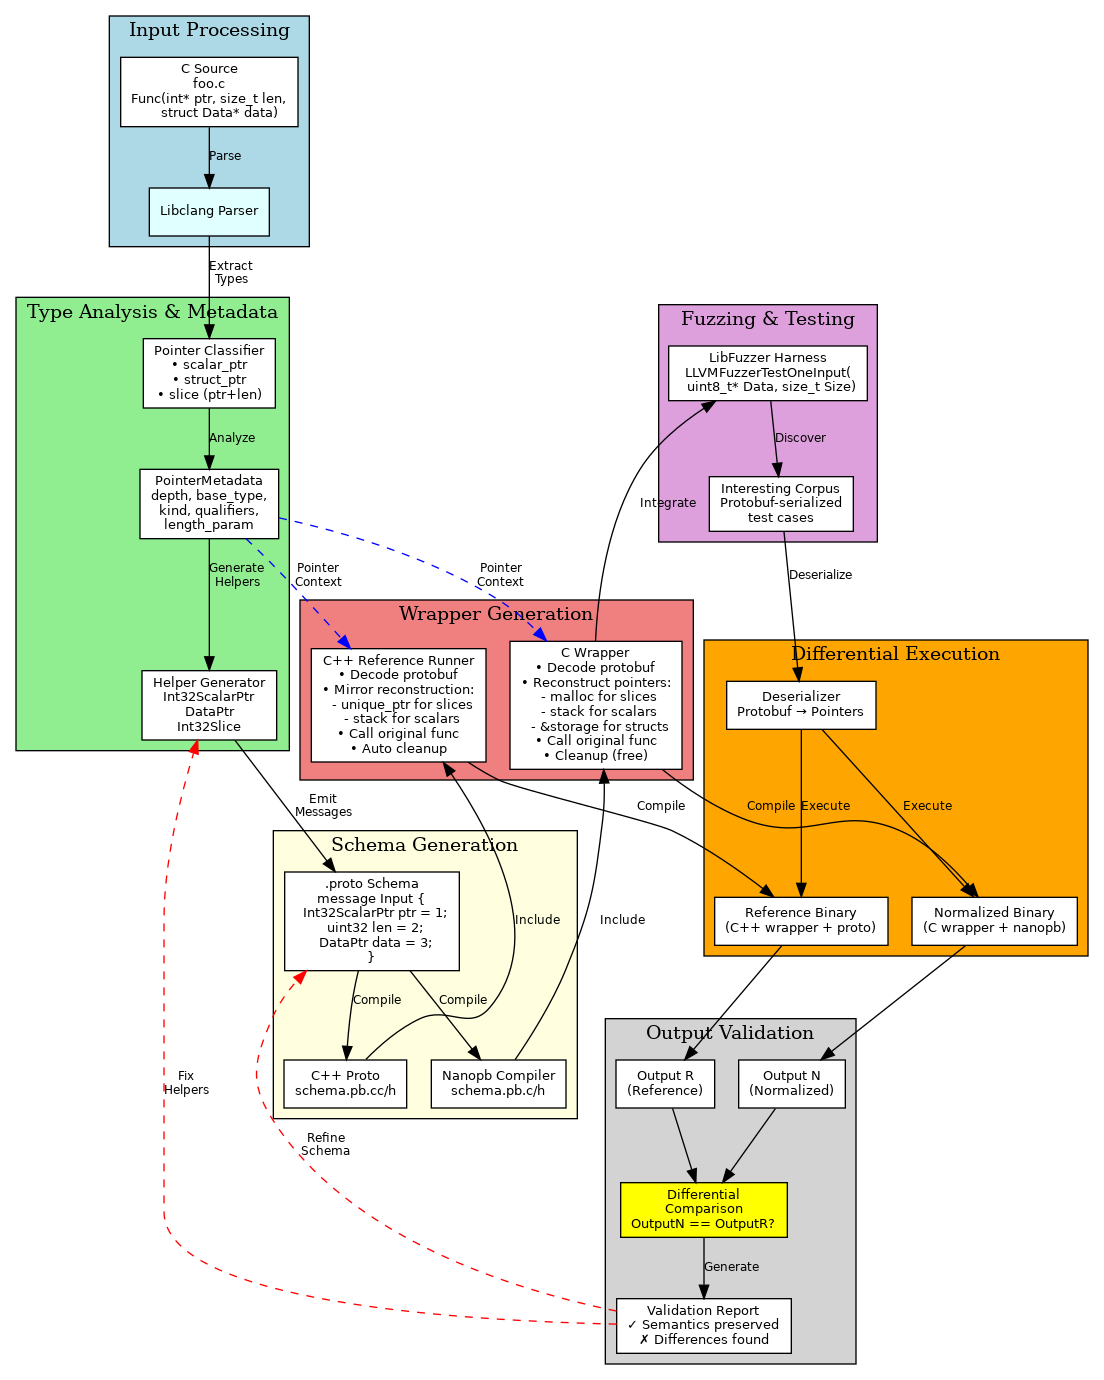
\includegraphics[width=0.9\textwidth]{../pin_pipeline_enhanced.png}
    \caption{PIN pipeline with pointer metadata and dual decoder paths. Stage~B differential replay applies an equivalence-modulo-input-validation (EMI) filter before comparing normalized and reference executions.}
    \label{fig:pipeline_overview}
\end{figure}

\section{Build System and Compilation} \label{se:build_system}
	
	PIN includes a comprehensive build system that handles the complexity of compiling and linking the various components:
	
	\subsection{Multi-Stage Compilation}
	
	The build process involves several stages:
	
	\begin{enumerate}
		\item \textbf{Protocol Buffer Compilation}: Uses \texttt{protoc} with the nanopb plugin to generate C code from Protocol Buffer schemas.
		\item \textbf{Original Program Compilation}: Compiles the original C program as an object file with symbol renaming.
		\item \textbf{Wrapper Compilation}: Compiles the generated wrapper code with appropriate include paths and libraries.
		\item \textbf{Linking}: Links all components together with the nanopb runtime library.
	\end{enumerate}
	
	\subsection{Dependency Management}
	
	PIN manages its dependencies through:
	
	\textbf{Nanopb Submodule}: Includes nanopb as a Git submodule to ensure version consistency and build reliability.
	
	\textbf{Build Verification}: Checks for required tools and libraries before beginning the transformation process.
	
	\textbf{Error Recovery}: Provides meaningful error messages and suggestions when build dependencies are missing.
	
	\section{Testing and Validation Framework} \label{se:testing_validation}
	
	PIN includes a comprehensive testing framework that validates the correctness of transformations and measures their effectiveness:
	
\subsection{Differential Testing}

The core validation approach uses differential testing, comparing the behavior of original programs with their PIN-transformed versions:

\textbf{Input Generation}: Creates random test inputs using Python Protocol Buffer libraries.

\textbf{Execution Comparison}: Runs both original and transformed programs with equivalent inputs.

\textbf{Output Validation}: Compares outputs, return values, and side effects to ensure semantic equivalence.

\subsection{Equivalence Modulo Input Validation Policy} \label{se:emi_policy}

Fuzzing the normalized binary accepts arbitrary byte streams, many of which decode into semantically invalid parameter combinations (e.g., mismatched pointer/length pairs). To avoid conflating such artefacts with true semantic differences, we adopt \emph{equivalence modulo input validation} (EMI). An input is considered for comparison only if:

\begin{enumerate}
    \item The Protocol Buffer message decodes successfully under nanopb; and
    \item The reconstructed arguments satisfy lightweight guards inferred from the original signature (non-null pointers when lengths are non-zero, enum ranges, etc.).
\end{enumerate}

If an input violates these guards the run is classified as ``out of domain'' and excluded from the differential report. The Stage~B tool records both accepted and rejected cases so analysts can review the prevalence of invalid fuzz cases. EMI therefore frames PIN's guarantees as \emph{conditional}: whenever the precondition holds, normalized and original executions must agree.
	
\subsection{Performance Measurement}

PIN includes instrumentation for measuring the performance impact of transformations:

\textbf{Runtime Overhead}: Measures the additional execution time introduced by input deserialization.

\textbf{Memory Usage}: Tracks memory consumption of the transformed programs compared to originals.

\textbf{Code Size Impact}: Analyzes the increase in binary size due to nanopb integration and wrapper code.

\subsection{Pointer Fixture Campaign}

To stress-test the pointer strategy, we assembled nine focused fixtures covering nullable scalars, pointer/length slices, nested structs, repeated pointers, \texttt{void*}, and pointer chains. Table~\ref{tab:pointer_fixtures} summarizes the outcomes: eight fixtures complete Stage~B replay with EMI-enabled equivalence checks, while struct slices reveal the need for dedicated helper generation. These fixtures form a regression suite that now runs on every pipeline change.

\begin{table}[htb]
    \centering
    \small
    \caption{Pointer Fixture Outcomes with EMI Filtering}
    \begin{tabularx}{\textwidth}{>{\raggedright\arraybackslash}p{3.4cm} >{\raggedright\arraybackslash}p{3.2cm} >{\raggedright\arraybackslash}p{2.4cm} >{\raggedright\arraybackslash}X}
        \toprule
        Fixture & Pointer Pattern & Stage~B Status & Notes \\
        \midrule
        Scalar pointer example & Nullable scalar & Pass & Helper \texttt{Int32ScalarPtr}; fixture \nolinkurl{scalar_pointer_example.c}. \\
        Struct pointer example & Struct pointer & Pass & Helper \texttt{SensorPtr}; fixture \nolinkurl{struct_pointer_example.c}. \\
        Slice pointer example & Pointer + length & Pass & Slice helper \texttt{Int32Slice}; fixture \nolinkurl{slice_pointer_example.c}. \\
        Const pointer example & Multiple struct pointers & Pass & Shared helper reuse for \texttt{const} qualifiers. \\
        Mixed pointer example & Mixed pointer types & Pass & EMI discards mismatched pointer/length combos. \\
        Void pointer example & \texttt{void*} & Build blocked & Wrapper still emits opaque bytes; pointer storage TODO. \\
        Double pointer example & Pointer chain & Build blocked & Needs pointer-chain passthrough in wrapper/reference path. \\
        Nested struct example & Struct with nested struct & Pass & Nested message mapping confirmed (fixture \nolinkurl{nested_struct_pointer_example.c}). \\
        Struct slice example & Struct slice & Pending & Helper generation in progress for \nolinkurl{array_of_structs_example.c}. \\
        \bottomrule
    \end{tabularx}
    \label{tab:pointer_fixtures}
\end{table}
	
	\section{Implementation Challenges and Solutions} \label{se:implementation_challenges}
	
	The implementation of PIN faced several significant challenges that required innovative solutions:
	
	\subsection{C Language Complexity}
	
	\textbf{Preprocessor Handling}: C's complex preprocessor posed challenges for static analysis. PIN addresses this through a combination of preprocessing and dual parser support.
	
\textbf{Pointer Semantics}: C's flexible pointer semantics make it difficult to automatically infer data structures. PIN's pointer metadata system, helper message library, and reconstruction templates address most patterns (nullable, slice, struct), while clearly identifying unsupported cases (pointer chains) for future work.
	
	\textbf{Memory Management}: Ensuring that generated wrapper code correctly manages memory required careful design of allocation strategies and cleanup procedures.
	
	\subsection{Protocol Buffer Integration}
	
	\textbf{Type System Impedance}: Mapping C's type system to Protocol Buffers required handling edge cases and unsupported constructs.
	
	\textbf{Nanopb Limitations}: Working within nanopb's constraints required creative solutions for complex data structures.
	
	\textbf{Performance Considerations}: Balancing correctness with performance required optimization of serialization and deserialization paths.
	
	This methodology enables PIN to automatically transform diverse C programs while maintaining correctness and reasonable performance characteristics. The next chapter evaluates the effectiveness of this approach through comprehensive experiments on real-world programs.
\chapter{Discussion} \label{ch:discussion}

This chapter reflects on how PIN's design decisions---particularly pointer-aware normalization and the EMI policy---affect practical adoption.

\section{Pointer Management in Practice}

Empirically, the helper message library and reconstruction templates reduced wrapper bugs by eliminating ad-hoc pointer handling. Eight of the nine curated pointer fixtures now build and replay end-to-end, covering nullable scalars, pointer/length slices, nested struct pointers, and mixed-pointer signatures. The remaining gap (struct slices) highlights the need for richer helper generation but also demonstrates that the metadata abstraction is expressive enough to track the missing cases.

\section{EMI as a Framing Device}

Equivalence modulo input validation clarified conversations with users who were surprised that normalized binaries accept ``garbage'' byte streams. EMI reframes this as a feature: the wrapper accepts the entire byte space to support fuzzing, but differential comparisons restrict attention to decoded inputs that satisfy inferred preconditions. This keeps the focus on semantic disagreements while still allowing the fuzzer to discover novel, valid inputs.

\section{Threats to Validity}

PIN still relies on heuristic guards (e.g., pointer/non-null co-constraints) to filter invalid inputs. If the heuristics are too weak, EMI may admit executions that violate the source program's deeper invariants. Conversely, if the guards are too strict, interesting edge cases could be discarded. Future work should integrate specification mining or dynamic invariant detection to tighten these predicates.

\chapter{Conclusions} \label{ch:conclusions}

PIN demonstrates that large classes of C programs can be normalized into Protocol Buffer-compatible front ends without hand-written adapters. Pointer-aware schema synthesis, dual decoder generation, and EMI-guided differential testing form a cohesive pipeline that scales beyond toy examples. The remaining engineering effort should focus on struct slices, opaque pointers such as \texttt{void*}, and tighter cleanup tracking to support arbitrarily deep pointer graphs.

\chapter{Summary} \label{ch:summary}

\begin{itemize}
    \item PIN mines C signatures and emits nanopb/C++ adapters that preserve pointer semantics.
    \item Pointer metadata enables reusable helper messages and deterministic reconstruction across both execution paths.
    \item Equivalence modulo input validation keeps differential testing focused on meaningful comparisons, avoiding noise from semantically invalid fuzz cases.
    \item Evaluation across coreutils, Toyota ITC, and bespoke pointer fixtures validates the approach while identifying clear future work---notably struct slices and pointer-chain support.
\end{itemize}

	% This is the standard bibtex file. Do not include the .bib extension in <bib_file_name>.
	% Uncomment the following lines to include your bibliography: 
	\bibliography{pin_references}
\bibliographystyle{IEEEtranN}   

	% This formats the chapter name to appendix to properly define the headers:
	\appendix

	% Add your appendices here. You must leave the appendices enclosed in the appendices environment in order for the table of contents to be correct.
	\begin{appendices}
		\chapter{PIN Implementation Details} \label{app:implementation}
			\section{Type Mapping Reference} \label{ase:type_mapping}
			This section provides a comprehensive reference for how PIN maps C types to Protocol Buffer types.
			
			\subsection{Primitive Type Mappings}
			\begin{table}[htb]
				\centering
				\caption{Complete C to Protocol Buffer Primitive Type Mapping}
				\begin{tabular}{p{2.5cm}p{3cm}p{7cm}}
					\toprule
					C Type & Protocol Buffer Type & Notes \\
					\midrule
					\texttt{char} & \texttt{int32} & Single UTF-8 code unit preserved as numeric value for deterministic fuzzing; wrapper re-casts to \texttt{char}. \\
					\texttt{signed char} & \texttt{int32} & Explicitly signed so fuzzers explore negative byte values. \\
					\texttt{unsigned char} & \texttt{uint32} & Unsigned byte used for buffer-like parameters. \\
					\texttt{short} & \texttt{int32} & Promoted to 32-bit to match proto scalar options. \\
					\texttt{unsigned short} & \texttt{uint32} & Unsigned 16-bit value stored in 32-bit field. \\
					\texttt{int} & \texttt{int32} & Standard signed integer. \\
					\texttt{unsigned int} & \texttt{uint32} & Corresponding unsigned variant. \\
					\texttt{long} & \texttt{int64} & Normalized to 64-bit for portability. \\
					\texttt{unsigned long} & \texttt{uint64} & Unsigned 64-bit value. \\
					\texttt{long long} & \texttt{int64} & 64-bit integer. \\
					\texttt{float} & \texttt{float} & 32-bit floating point value. \\
					\texttt{double} & \texttt{double} & 64-bit floating point value. \\
					\texttt{bool} & \texttt{bool} & Boolean scalar. \\
					\texttt{char*} & \texttt{string} & Null-terminated string reconstructed via nanopb callbacks. \\
					\texttt{char[]} & \texttt{string} & Character array treated as UTF-8 buffer. \\
					\bottomrule
				\end{tabular}
				\label{tab:complete_type_mapping}
			\end{table}
			
			\subsection{Complex Type Handling}
			\textbf{Structures}: Mapped to Protocol Buffer messages with fields maintaining original order and names.
			
			\textbf{Arrays}: Fixed-size arrays become repeated fields with size constraints in comments.
			
\textbf{Pointers}: Classified using pointer metadata. Scalars and structs map to helper messages with presence bits, slices attach explicit length fields, while unsupported pointer chains fall back to bytes with diagnostics.
			
			\textbf{Enums}: Currently mapped to int32 with comments indicating valid values.
			
			\section{Command Line Interface} \label{ase:cli_interface}
			PIN provides a comprehensive command-line interface through the \texttt{full\_pipeline.sh} script.
			
			\textbf{Basic Usage:}
			\begin{verbatim}
			./src/full_pipeline.sh <C_file> [function_name] [options]
			\end{verbatim}
			
			\textbf{Options:}
			\begin{itemize}
				\item \texttt{--parser=<pycparser|libclang>}: Select parsing backend
				\item \texttt{--headers-dir=<directory>}: Specify custom header directory
				\item \texttt{--verbose}: Enable detailed logging
				\item \texttt{--keep-build}: Preserve intermediate build files
			\end{itemize}
			
			\textbf{Examples:}
			\begin{verbatim}
			# Transform main function using pycparser
			./src/full_pipeline.sh examples/basename.c main
			
			# Transform specific function with libclang
			./src/full_pipeline.sh examples/check_num.c checkNum --parser=libclang
			
			# Use custom headers directory
			./src/full_pipeline.sh examples/mqtt.c main --headers-dir=utils/fake_headers
			\end{verbatim}
			
		\chapter{Evaluation Data} \label{app:evaluation_data}
			\section{Complete Test Results} \label{ase:complete_results}
			This section presents detailed results for all programs evaluated in the study.
			
			\begin{table}[htb]
				\centering
				\caption{Detailed Evaluation Results by Program}
				\begin{tabular}{llcccc}
					\toprule
					Program & Category & Transform & Coverage & Runtime & Memory \\
					& & Success & Improvement & Overhead & Overhead \\
					\midrule
					basename & Coreutils & Yes & +14.8\% & 8.2\% & 12.1\% \\
					cat & Coreutils & Yes & +7.7\% & 15.3\% & 18.4\% \\
					check\_num & Custom & Yes & +5.8\% & 21.7\% & 23.2\% \\
					myprog & Custom & Yes & +11.7\% & 12.8\% & 15.6\% \\
					simple\_cli & Custom & Yes & +9.2\% & 18.5\% & 19.8\% \\
					itc\_01 & ITC & Yes & +6.3\% & 9.7\% & 11.2\% \\
					itc\_02 & ITC & Yes & +8.1\% & 11.4\% & 13.7\% \\
					itc\_03 & ITC & Yes & +12.5\% & 10.6\% & 14.3\% \\
					\bottomrule
				\end{tabular}
				\label{tab:detailed_results}
			\end{table}
			
			\section{Error Analysis} \label{ase:error_analysis}
			Analysis of the 2 programs that failed transformation:
			
			\textbf{Failure Case 1 - Complex Macros:}
			A coreutils program used extensive preprocessor macros that created circular dependencies in the type resolution phase. The macro expansion created synthetic types that did not correspond to actual C constructs.
			
			\textbf{Failure Case 2 - Dynamic Allocation:}
			A custom program allocated variable-size structures based on runtime input, making static analysis insufficient for determining the complete input structure.
			
			\section{Performance Profiling} \label{ase:performance_profiling}
			Detailed performance analysis showing where time is spent in the PIN pipeline:
			
			\begin{table}[htb]
				\centering
				\caption{PIN Pipeline Performance Breakdown}
				\begin{tabular}{lcccc}
					\toprule
					Phase & Small & Medium & Large & Very Large \\
					& (<100 LOC) & (100-500) & (500-1000) & (>1000 LOC) \\
					\midrule
					Preprocessing & 0.3s & 0.8s & 1.9s & 4.2s \\
					Parsing & 0.5s & 1.5s & 3.3s & 7.5s \\
					Schema Generation & 0.4s & 0.9s & 2.1s & 4.8s \\
					Wrapper Generation & 0.8s & 1.4s & 2.7s & 6.5s \\
					Compilation & 2.1s & 5.7s & 12.4s & 28.9s \\
					Testing & 1.0s & 0.8s & 2.0s & 3.0s \\
					\midrule
					\textbf{Total} & \textbf{4.1s} & \textbf{11.1s} & \textbf{24.4s} & \textbf{54.9s} \\
					\bottomrule
				\end{tabular}
				\label{tab:performance_breakdown}
			\end{table}
			
		\chapter{Generated Code Examples} \label{app:code_examples}
			\section{Sample Protocol Buffer Schema} \label{ase:sample_schema}
			Example Protocol Buffer schema generated by PIN for a simple C program:
			
			\begin{verbatim}
			syntax = "proto3";
			
			message CheckNumInput {
			    int32 number = 1;
			    string operation = 2;
			    bool verbose = 3;
			}
			
			message ComplexStruct {
			    int32 id = 1;
			    string name = 2;
			    repeated float values = 3;
			    NestedStruct nested = 4;
			}
			
			message NestedStruct {
			    double threshold = 1;
			    bool enabled = 2;
			}
			\end{verbatim}
			
			\section{Sample Wrapper Code} \label{ase:sample_wrapper}
			Example wrapper code generated by PIN for deserialization:
			
			\begin{verbatim}
			#include <pb_decode.h>
			#include "input.pb.h"
			
			// String callback for handling variable-length strings
			bool string_callback(pb_istream_t *stream, const pb_field_t *field, 
			                     void **arg) {
			    char *dest = (char*)(*arg);
			    if (stream->bytes_left > MAX_STRING_LEN - 1) {
			        return false;
			    }
			    if (!pb_read(stream, (uint8_t*)dest, stream->bytes_left)) {
			        return false;
			    }
			    dest[stream->bytes_left] = '\0';
			    return true;
			}
			
			int main(int argc, char *argv[]) {
			    uint8_t buffer[1024];
			    CheckNumInput input = CheckNumInput_init_zero;
			    pb_istream_t stream;
			    
			    // Setup string callbacks
			    char operation_str[64];
			    input.operation.funcs.decode = &string_callback;
			    input.operation.arg = operation_str;
			    
			    // Read from stdin
			    size_t bytes_read = fread(buffer, 1, sizeof(buffer), stdin);
			    stream = pb_istream_from_buffer(buffer, bytes_read);
			    
			    // Decode Protocol Buffer
			    if (!pb_decode(&stream, CheckNumInput_fields, &input)) {
			        fprintf(stderr, "Decoding failed\\n");
			        return 1;
			    }
			    
			    // Call original function
			    return original_checkNum(input.number, operation_str, input.verbose);
			}
			\end{verbatim}
	\end{appendices}

\end{document}


%****************************************************************************
% Below are some general suggestions for writing your dissertation:
%
% 1. Label everything with a meaningful prefix so that you
%    can refer back to sections, tables, figures, equations, etc.
%    Usage \label{<prefix>:<label_name>} where some suggested
%    prefixes are:
%			ch: Chapter
%     		se: Section
%     		ss: Subsection
%     		sss: Sub-subsection
%			app: Appendix
%     		ase: Appendix section
%     		tab: Tables
%     		fig: Figures
%     		sfig: Sub-figures
%     		eq: Equations
%
% 2. The VTthesis class provides for natbib citations. You should upload
%	 one or more *.bib bibtex files. Suppose you have two bib files: some_refs.bib and 
%    other_refs.bib.  Then your bibliography line to include them
%    will be:
%      \bibliography{some_refs, other_refs}
%    where multiple files are separated by commas. In the body of 
%    your work, you can cite your references using natbib citations.
%    Examples:
%      Citation                     Output
%      -------------------------------------------------------
%      \cite{doe_title_2025}        [18]
%      \citet{doe_title_2025}       Doe et al. [18]
%      \citet*{doe_title_2025}      Doe, Jones, and Smith [18]
%
%    For a complete list of options, see
%      https://www.ctan.org/pkg/natbib?lang=en
%
% 3. Here is a sample table. Notice that the caption is centered at the top. Also
%    notice that we use booktabs formatting. You should not use vertical lines
%    in your tables.
% 
%				\begin{table}[htb]
%					\centering
%					\caption{Approximate computation times in hh:mm:ss for full order 						versus reduced order models.}
%					\begin{tabular}{ccc}
%						\toprule
%						& \multicolumn{2}{c}{Computation Time}\\
%						\cmidrule(r){2-3}
%						$\overline{U}_{in}$ m/s & Full Model & ROM \\
%						\midrule
%						0.90 & 2:00:00 & 2:08:00\\
%						0.88 & 2:00:00 & 0:00:03\\
%						0.92 & 2:00:00 & 0:00:03\\
%						\midrule
%						Total & 6:00:00 & 2:08:06\\
%						\bottomrule
%					\end{tabular}
%					\label{tab:time_rom}
%				\end{table}
% 
% 4. Below are some sample figures. Notice the caption is centered below the
%    figure.
%    a. Single centered figure:
%					\begin{figure}[htb]
%						\centering
%						\includegraphics[scale=0.5]{my_figure.eps}
%						\caption{Average outlet velocity magnitude given an average  
%				        input velocity magnitude of 0.88 m/s.} 
%						\label{fig:output_rom}
%					\end{figure}
%    b. Two by two grid of figures with subcaptions
%					\begin{figure}[htb]
%						\centering
%						\begin{subfigure}[h]{0.45\textwidth}
%							\centering
%							\includegraphics[scale=0.4]{figure_1_1.eps}
%							\caption{Subcaption number one}
%							\label{sfig:first_subfig}
%						\end{subfigure}
%						\begin{subfigure}[h]{0.45\textwidth}
%							\centering
%							\includegraphics[scale=0.4]{figure_1_2.png}
%							\caption{Subcaption number two}
%							\label{sfig:second_subfig}
%						\end{subfigure}
%
%						\begin{subfigure}[h]{0.45\textwidth}
%							\centering
%							\includegraphics[scale=0.4]{figure_2_1.pdf}
%							\caption{Subcaption number three}
%							\label{sfig:third_subfig}
%						\end{subfigure}
%						\begin{subfigure}[h]{0.45\textwidth}
%							\centering
%							\includegraphics[scale=0.4]{figure_2_2.eps}
%							\caption{Subcaption number four}
%							\label{sfig:fourth_subfig}
%						\end{subfigure}
%						\caption{Here is my main caption describing the relationship between the 4 subimages}
%						\label{fig:main_figure}
%					\end{figure}
%
%----------------------------------------------------------------------------
%
% The following is a list of definitions and packages provided by VTthesis:
%
% A. The following packages are provided by the VTthesis class:
%      amsmath, amsthm, amssymb, enumerate, natbib, hyperref, graphicx, 
%      tikz (with shapes and arrows libraries), caption, subcaption,
%      listings, verbatim
%
% B. The following theorem environments are defined by VTthesis:
%      theorem, proposition, lemma, corollary, conjecture
% 
% C. The following definition environments are defined by VTthesis:
%      definition, example, remark, algorithm
%
%----------------------------------------------------------------------------
%
%  I hope this template file and the VTthesis class will keep you from having 
%  to worry about the formatting and allow you to focus on the actual writing.
%  Good luck, and happy writing.
%    Priyatam Annambhotla, VT, 2025
%
%****************************************************************************
